% compile with: pdflatex -shell-escape filename.tex
\documentclass[crop,tikz,convert=pdf2svg]{standalone}
\usepackage{forest}
\usetikzlibrary{matrix}

\begin{document}

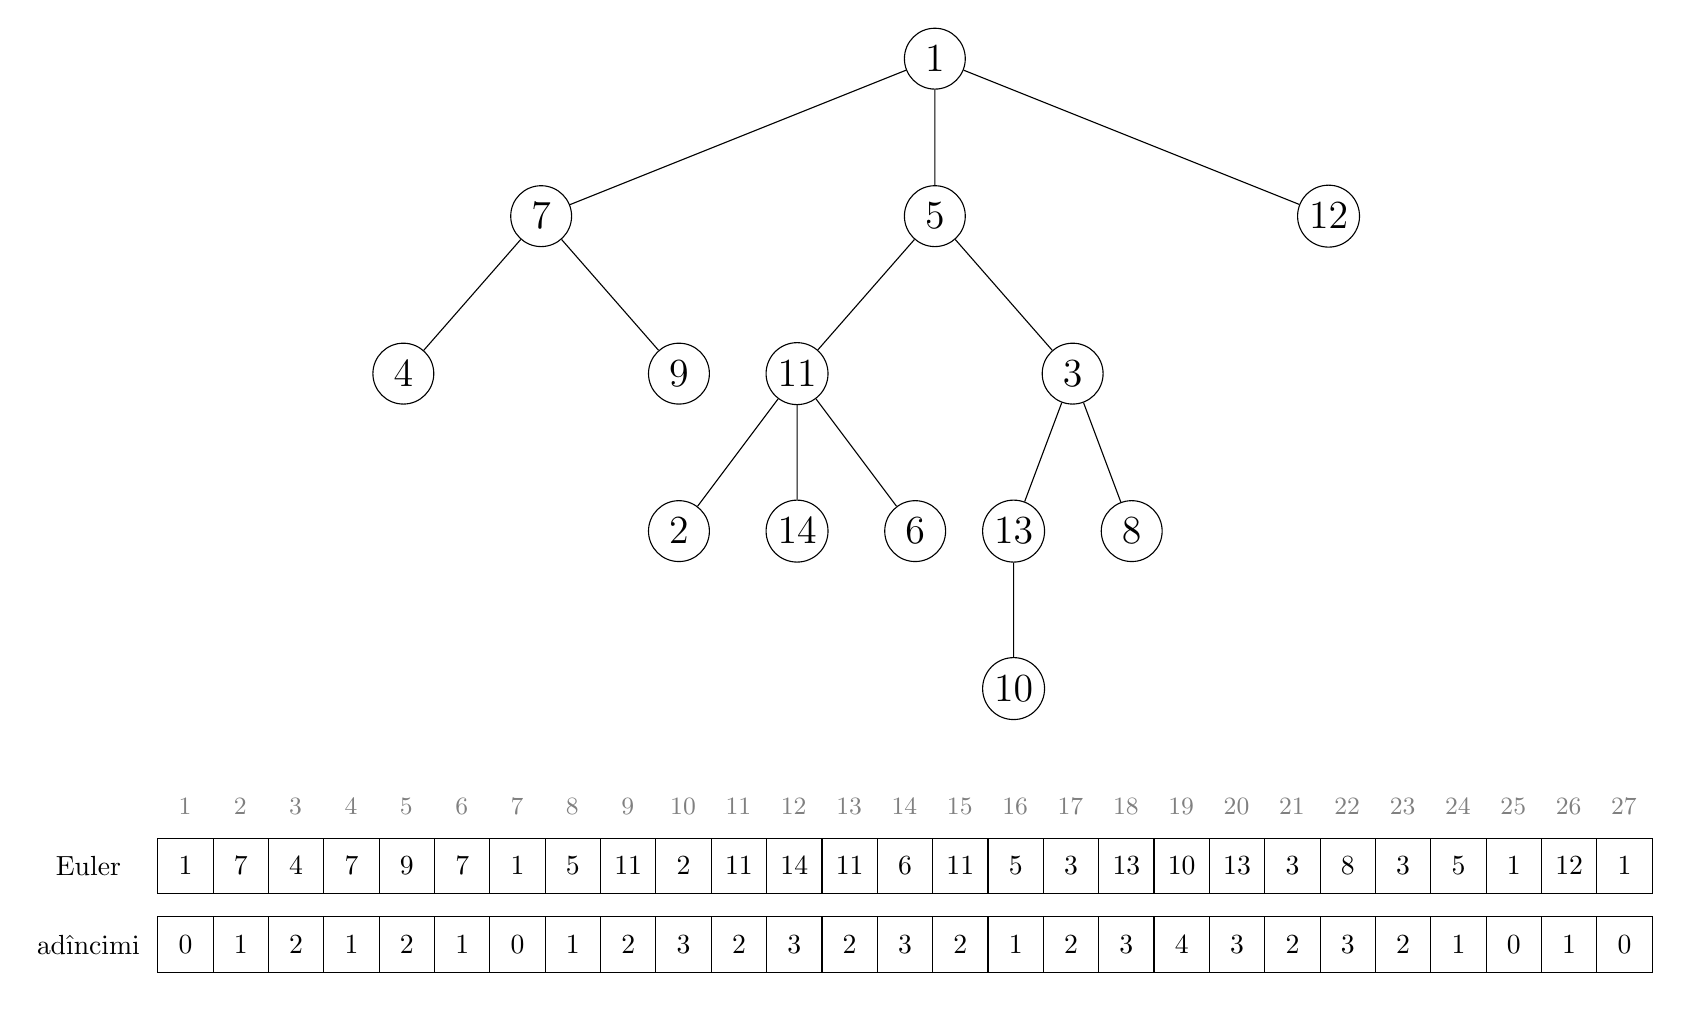
\begin{tikzpicture}
  \begin{scope}[
      every node/.style={
        circle,
        draw,
        font=\Large,
        inner sep=2pt,
        minimum size=22pt,
      },
      level distance=20mm,
      level 1/.style={sibling distance=50mm},
      level 2/.style={sibling distance=35mm},
      level 3/.style={sibling distance=15mm}
    ]
    \node {1}
    child {node {7}
      child {node {4}}
      child {node {9}}
    }
    child {node {5}
      child {node {11}
        child {node {2}}
        child {node {14}}
        child {node {6}}
      }
      child {node {3}
        child {node {13}
          child {node {10}}
        }
        child {node {8}}
      }
    }
    child {node {12}};
  \end{scope}

  \begin{scope}[shift={(-10,-9.5)}]
    % First row: indices
    \matrix[right] (index) at (0, 0) [
      matrix of nodes,
      nodes={anchor=center, minimum size=20pt, color=black!50, font=\small},
    ] {
      1 & 2 & 3 & 4 & 5 & 6 & 7 & 8 & 9 & 10 & 11 & 12 & 13 & 14 & 15 & 16 &
      17 & 18 & 19 & 20 & 21 & 22 & 23 & 24 & 25 & 26 & 27\\
    };

    % Second row: Euler linearization
    \node[label] (label-abstract) at (-0.75, -0.75) {Euler};

    \matrix[right] (abstract) at (0, -0.75) [
      matrix of nodes,
      nodes={draw, anchor=center, minimum size=20pt},
      column sep=-\pgflinewidth,
      row sep=-\pgflinewidth
    ] {
      1 & 7 & 4 & 7 & 9 & 7 & 1 & 5 & 11 & 2 & 11 & 14 & 11 & 6 & 11 & 5 & 3 &
      13 & 10 & 13 & 3 & 8 & 3 & 5 & 1 & 12 & 1\\
    };

    % Third row: depths
    \node[label] (label-abstract) at (-0.75, -1.75) {adîncimi};

    \matrix[right] (abstract) at (0, -1.75) [
      matrix of nodes,
      nodes={draw, anchor=center, minimum size=20pt},
      column sep=-\pgflinewidth,
      row sep=-\pgflinewidth
    ] {
      0 & 1 & 2 & 1 & 2 & 1 & 0 & 1 & 2 & 3 & 2 & 3 & 2 & 3 & 2 & 1 & 2 & 3 &
      4 & 3 & 2 & 3 & 2 & 1 & 0 & 1 & 0\\
    };
  \end{scope}
\end{tikzpicture}

\end{document}
